\ac{rag} has emerged as the principal architectural pattern to mitigate the inherent limitations of standalone \acp{llm} \cite{SOTA-RAG-SURVEY}. While \acp{llm} offer powerful reasoning and language generation capabilities, their reliance on static, internal knowledge leads to several challenges for recommendation tasks:
\begin{compactitem}[\textbullet]
    \item \textbf{Knowledge cut-off:} The model is unaware of any items, events, or information created after its training date, making it incapable of recommending new or timely content.
    \item \textbf{Hallucination:} \acp{llm} are prone to generating factually incorrect or entirely fabricated information, which can severely erode user trust if the system suggests non-existent items or attributes.
    \item \textbf{Lack of domain awareness:} A general-purpose model has no specific knowledge of a particular service's inventory, such as which products are in stock or their current prices.
    \item \textbf{Difficulty leveraging behavioral data:} The rich collaborative signals from user-item interactions (e.g., ratings, purchases) are not naturally represented in the parametric knowledge of an \ac{llm}.
\end{compactitem}

\ac{rag} directly addresses these issues by grounding the \ac{llm} in an external, authoritative knowledge base. The standard workflow, consists of an offline indexing stage and an online retrieval-generation stage, with the latter depicted in Figure~\ref{FIG:RAG_WORKFLOW}. During indexing, documents are cleaned, segmented into chunks, converted into vector embeddings, and stored in a vector database. At runtime, a user's query is embedded and used to retrieve the most relevant chunks, which are then passed to the \ac{llm} as context to generate a factually grounded response.

\begin{figure}[RAG Workflow]{FIG:RAG_WORKFLOW}{The standard \acl{rag} workflow \cite{AWS-RAG}.}
    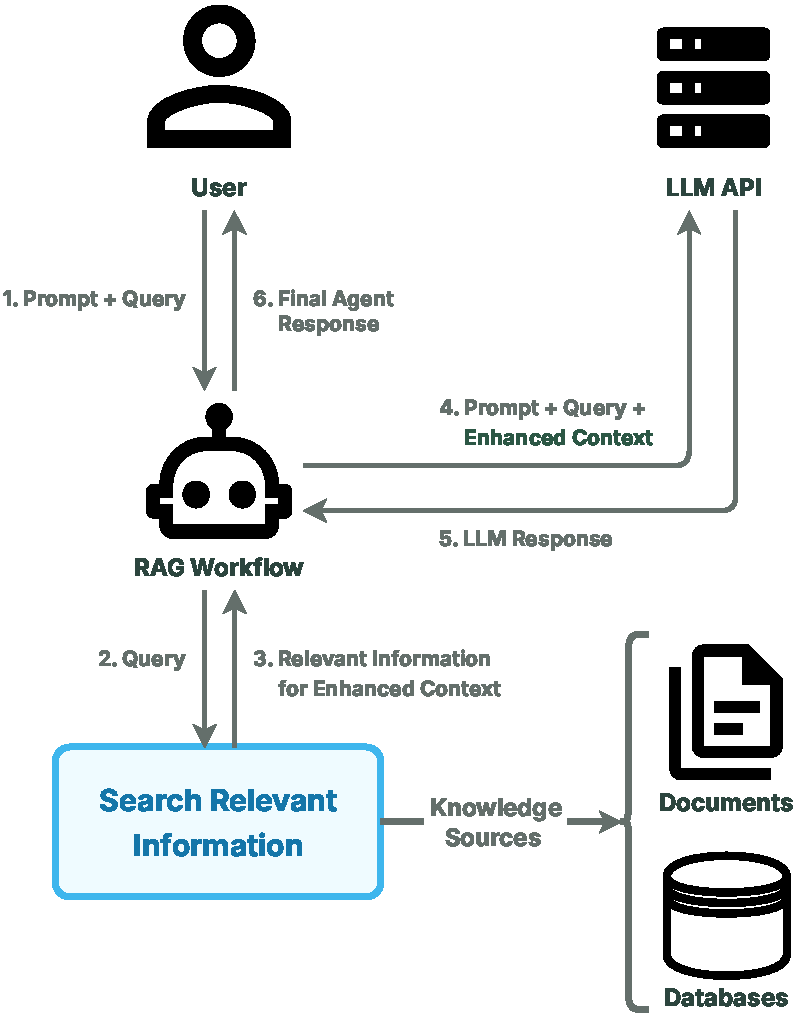
\includegraphics[width=0.52\textwidth]{rag_workflow.pdf}
\end{figure}

The application of \ac{rag} is evolving beyond simple fact retrieval into a more sophisticated paradigm, with advanced techniques to further address the limitations of traditional \acp{llm} \cite{SOTA-ADVANCED-RAG}. This has led to the development of \textbf{Graph-\ac{rag}} \cite{GRAPHRAG-CRS}, where the retrieval source is a structured \ac{kg} that stores relevant information as nodes and relationships. The initial use of \ac{rag} was as a ``fact-checker'' to provide domain awareness and prevent hallucinations. However, state-of-the-art research in \ac{rag} applied to \ac{crs} now conceptualizes \ac{rag} as a \textit{collaborative signal retriever}. The goal is to retrieve not just item descriptions, but the complex, relational data that powers traditional \acl{cf}. By applying Graph-\ac{rag}, this model allows the system to query for explicit reasoning paths. Frameworks like \texttt{G-Refer} \cite{G-REFER} and \texttt{CRAG} \cite{COLLAB-LLM-CRS} exemplify this approach, using graph traversal to find evidence that is then translated into natural language by the \ac{llm} to generate a recommendation and a faithful explanation.